\section{Architectural Details}

The main idea of the Inception architecture is based on finding out how an optimal local sparse structure in a convolutional vision network can be approximated and covered by readily available dense components. Note that assuming translation invariance means that our network will be built from convolutional building blocks. All we need is to find the optimal local construction and to repeat it spatially. Arora et al.~\cite{arora2013bounds} suggests a layer-by layer construction in which one should analyze the correlation statistics of the last layer and cluster them into groups of units with high correlation. These clusters form the units of the next layer and are connected to the units in the previous layer. We assume that each unit from the earlier layer corresponds to some region of the input image and these units are grouped into filter banks. In the lower layers (the ones close to the input) correlated units would concentrate in local regions. This means, we would end up with a lot of clusters concentrated in a single region and they can be covered by a layer of $1{\times}1$ convolutions in the next layer, as suggested in ~\cite{lin2013nin}. However, one can also expect that there will be a smaller number of more spatially spread out clusters that can be covered by convolutions over larger patches, and there will be a decreasing number of patches over larger and larger regions. In order to avoid patch-alignment issues, current incarnations of the Inception architecture are restricted to filter sizes $1{\times}1$, $3{\times}3$ and $5{\times}5$, however this decision was based more on convenience rather than necessity. It also means that the suggested architecture is a combination of all those layers with their output filter banks concatenated into a single output vector forming the input of the next stage. Additionally, since pooling operations have been essential for the success in current state of the art convolutional networks, it suggests that adding an alternative parallel pooling path in each such stage should have additional beneficial effect, too (see Figure~\ref{fig:inceptionnaive}).

\begin{figure}
\centering
\subfigure[Inception module, na\"{i}ve version]{
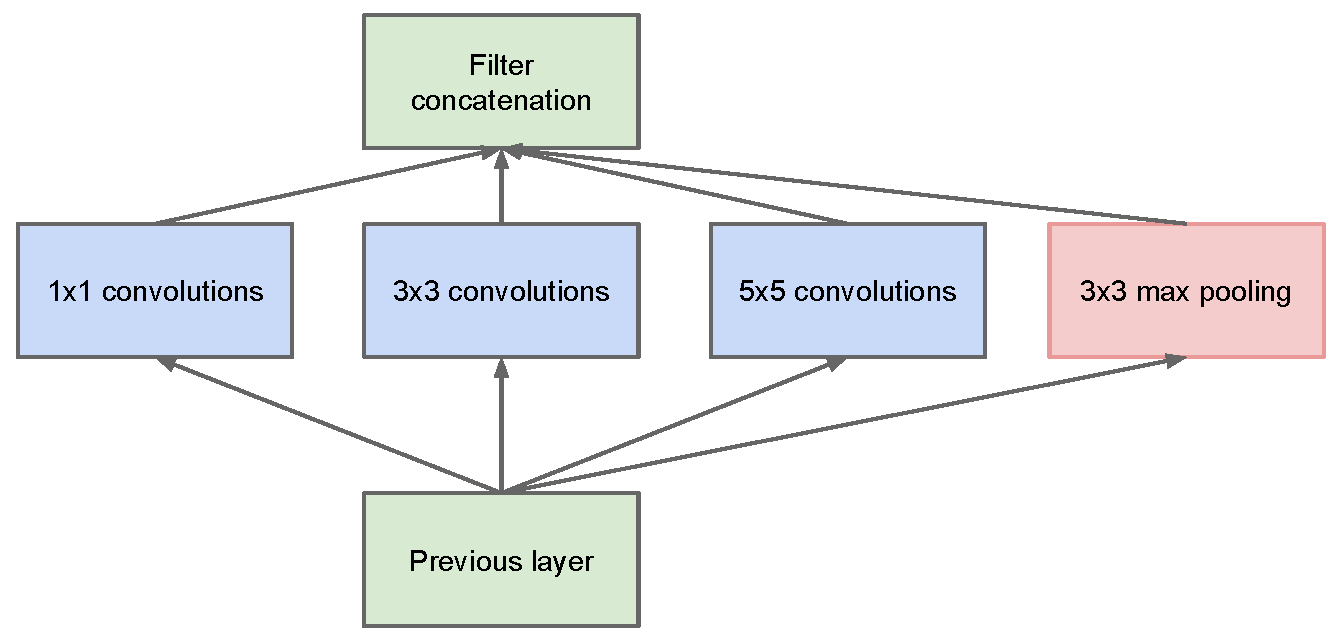
\includegraphics[width=0.48\textwidth]{inceptionnaive.pdf}
\label{fig:inceptionnaive}
}
\subfigure[Inception module with dimension reductions]{
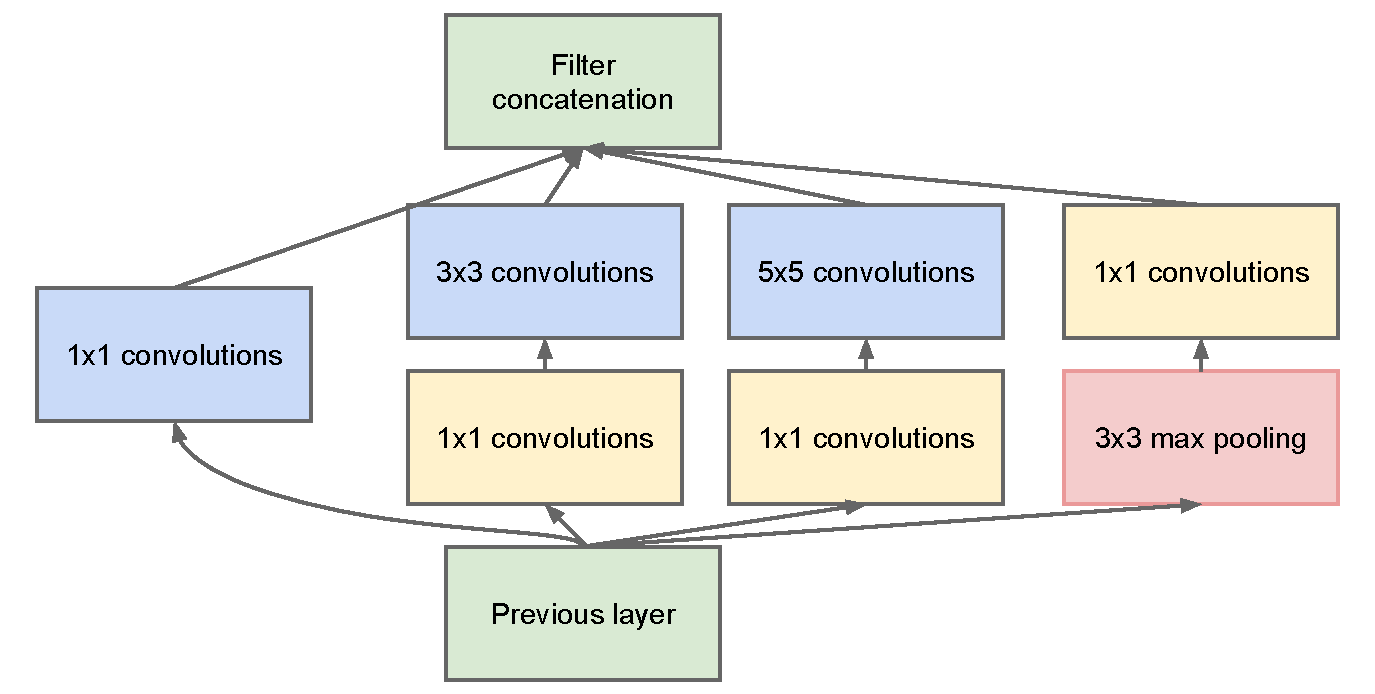
\includegraphics[width=0.48\textwidth]{inceptionmodule.pdf}
\label{fig:inceptionmodule}
}
\caption{Inception module}
\label{fig:inception}
\end{figure}

As these ``Inception modules'' are stacked on top of each other, their output correlation statistics are bound to vary: as features of higher abstraction are captured by higher layers, their spatial concentration is expected to decrease suggesting that the ratio of $3{\times}3$ and $5{\times}5$ convolutions should increase as we move to higher layers. 

One big problem with the above modules, at least in this na\"{i}ve form, is that even a modest number of $5{\times}5$ convolutions can be prohibitively expensive on top of a convolutional layer with a large number of filters. This problem becomes even more pronounced once pooling units are added to the mix: their number of output filters equals to the number of filters in the previous stage. The merging of the output of the pooling layer with the outputs of convolutional layers would lead to an inevitable increase in the number of outputs from stage to stage. Even while this architecture might cover the optimal sparse structure, it would do it very inefficiently, leading to a computational blow up within a few stages. 

This leads to the second idea of the proposed architecture: judiciously applying dimension reductions and projections wherever the computational requirements would increase too much otherwise. This is based on the success of embeddings: even low dimensional embeddings might contain a lot of information about a relatively large image patch. However, embeddings represent information in a dense, compressed form and compressed information is harder to model. We would like to keep our representation sparse at most places (as required by the conditions of ~\cite{arora2013bounds}) and compress the signals only whenever they have to be aggregated en masse. That is, $1{\times}1$ convolutions are used to compute reductions before the expensive $3{\times}3$ and $5{\times}5$ convolutions. Besides being used as reductions, they also include the use of rectified linear activation which makes them dual-purpose. The final result is depicted in Figure~\ref{fig:inceptionmodule}.

In general, an Inception network is a network consisting of modules of the above type stacked upon each other, with occasional max-pooling layers with stride 2 to halve the resolution of the grid. For technical reasons (memory efficiency during training), it seemed beneficial to start using Inception modules only at higher layers while keeping the lower layers in traditional convolutional fashion. This is not strictly necessary, simply reflecting some infrastructural inefficiencies in our current implementation.

One of the main beneficial aspects of this architecture is that it allows for increasing the number of units at each stage significantly without an uncontrolled blow-up in computational complexity. The ubiquitous use of dimension reduction allows for shielding the large number of input filters of the last stage to the next layer, first reducing their dimension before convolving over them with a large patch size. Another practically useful aspect of this design is that it aligns with the intuition that visual information should be processed at various scales and then aggregated so that the next stage can abstract features from different scales simultaneously.

The improved use of computational resources allows for increasing both the width of each stage as well as the number of stages without getting into computational difficulties. Another way to utilize the inception architecture is to create slightly inferior, but computationally cheaper versions of it. We have found that all the included the knobs and levers allow for a controlled balancing of computational resources that can result in networks that are $2-3{\times}$ faster than similarly performing networks with non-Inception architecture, however this requires careful manual design at this point.
